%\RequirePackage{ifpdf}
\pdfoutput=1
\documentclass[cits]{JINST}
\usepackage{amsmath}
\let\ifpdf\relax

\title{21-channel imaging electron density interferometer}

\author{F. Glass\thanks{Corresponding
author.}, J. Howard, S. R. Haskey, C. A. Michael~and B.D. Blackwell\\
\llap{$$}Plasma Research Laboratory, The Australian National University\\
  Canberra ACT 0200 Australia\\
  E-mail: \email{fenton.glass@anu.edu.au}}

\abstract{
A novel 21-channel imaging interferometer for plasma density
measurements has been designed, installed, and commissioned on the H-1 heliac.
The new system replaces older, spatially-scanning interferometer systems\cite{WARR1997,HOWARD1992:2,HOWARD2006}, with an improvement in the temporal resolution from 1\ts{}ms to 10\ts{}$\mu$s.
In this article we report the design and technical innovations required to construct a plasma phase-imaging, millimeter-wave interferometer.
Guided by FDTD simulations of the wave propagation and diffraction, extensive system testing, using various corrugated targets, has confirmed diffraction-limited spatial resolution and excellent imaging fidelity in the presence of strong phase gradients.
}

\keywords{Plasma diagnostics - interferometry and imaging}

%%%%% some definitions %%%%%%
\def\be{\begin{equation}}
\def\ee{\end{equation}}
\def\bea{\begin{eqnarray}}
\def\eea{\end{eqnarray}}
\def\bd{\begin{description}}
\def\ed{\end{description}}
\def\bi{\begin{itemize}}
\def\ei{\end{itemize}}
\def\bc{\begin{center}}
\def\ec{\end{center}}

\def\non{\nonumber}
\def\infint{\int_{-\infty}^{\infty}}
\def\dinfint{\int\!\!\int_{-\infty}^{\infty}}
\def\bm#1{\mbox{\boldmath ${#1}$}}
\def\deg#1{${#1}^{\rm o}$}
\def\mod#1{\mid \! {#1} \! \mid}
\def\abs#1{\mid\!\! {#1} \!\! \mid}
\def\norm#1{\parallel {#1}\parallel}
\def\mean#1{\langle {#1}\rangle}
\def\eq#1{Eq. ({#1})}
\def\vol#1{\underbar{#1}}
\def\notll{\ll\!\!\!\!\!\! /\,\,\,\,\,}
\def\lsimeq{\;\raise.6ex\hbox{$<$}\mskip-13.5mu\lower.6ex\hbox{$\sim$}\;}
\def\gsimeq{\;\raise.6ex\hbox{$>$}\mskip-13.5mu\lower.6ex\hbox{$\sim$}\;}
\def\etal{{\it et al. }}


\def\apriori{{\it a priori }}
\def\aposteriori{{\it a posteriori }}
\def\prll{\parallel}
\def\eq#1{Eq.~(\ref{#1})}
\def\Fig#1{Fig.~\ref{#1}}
\def\fig#1{Fig.~\ref{#1}}

\def\curl{\nabla {\bm \times}}
\def\grad{\nabla}
\def\div{\nabla {\bm .}}
\def\idot{\bm .}
\def\cross{\bm \times}
\def\deriv#1{\stackrel{\bm .}{#1}}
\def\ds#1{\displaystyle #1}
\def\ne{n_{\rm e}}
\def\w0{{{{\rm w}}_0}}
\def\w{{\rm w}}
\def\bn{{\bm n}}
\def\bC{{\bm C}}
\def\bc{{\bm c}}
\def\bN{{\bm N}}
\def\bH{{\bm H}}
\def\un{\hat{\bm n}}
\def\ui{\hat{\bm i}}
\def\uj{\hat{\bm j}}
\def\uk{\hat{\bm k}}
\def\utheta{\hat{\bm \theta}}
\def\uphi{\hat{\bm phi}}
\def\ur{\hat{\bm r}}
\def\uz{\hat{\bm z}}
\def\uB{\hat{\bm B}}
\def\utheta{\hat{\bm \theta}}
\def\bB{{\bm B}}
\def\bD{{\bm D}}
\def\bT{{\bm T}}
\def\bw{{\bm w}}
\def\bW{{\bm W}}
\def\bp{{\bm p}}
\def\bP{{\bm P}}
\def\bq{{\bm q}}
\def\p{{u}}
\def\l{{\bm l}}
\def\t{{\rm t}}
\def\cbar{\bar{c}}
\def\Cbar{\bar{C}}
\def\c{{\rm c}}
\def\d{{\rm d}}
\def\s{{\rm s}}
\def\sn{{\eta }}
\def\dn{{\xi }}
\def\u{{\bm u}}
\def\U{{\bm U}}
\def\v{{\bm v}}
\def\V{{\bm V}}
\def\Q{{\bm Q}}
\def\t{{\rm t}}
\def\Ne{N_{\rm e}}
\def\me{m_{\rm e}}
\def\re{r_{\rm e}}
\def\ncr{n_{\rm cr}}
\def\lo#1{{#1}_{\rm LO}}
\def\r{{\bm r} }
\def\bkap{ {\bm \kappa} }
\def\brho{ {\bm \rho} }
\def\bsig{ {\bm \sig} }
\def\kaperp{ {{\bm \kappa}_{\perp}} }
\def\Kperp{ {{\bm K}_{\perp}} }
\def\kperp{ {{\bm k}_{\perp}} }
\def\kperpr{ {{\bm k}^{\prime }_{\perp}} }
\def\Kperpr{ {{\bm K}^{\prime }_{\perp}} }
\def\q{{\bm q} }
\def\bs{{\bm s} }
\def\R{{\bm R} }
\def\E{{\bm E} }
\def\bE{{\bm E} }
\def\bEperp{ {{\bm E}_{\perp} } }
\def\bvperp{ {{\bm v}_{\perp} } }
\def\buperp{ {{\bm u}_{\perp} } }
\def\D{{\bm D} }
\def\K{{\bm K} }
\def\k0{{\bm k}_0}
\def\ks{{\bm k}_{\rm s}}
\def\k{{\bm k}}
\def\z{{\bm z}}
\def\ulo{u_{\rm LO}}
\def\lens{\alpha}
\def\mix{r}
\def\avb{\mbox{$<\!\!\beta\!\!>$}}
\def\avg#1{\mbox{$<\!\!#1\!\!>$}}					 	
\def\Evec{{\bm E}}
\def\Fvec{{\bm F}}
\def\jvec{{\bm j}}
\def\kvec{{\bm k}}
\def\vvec{{\bm v}}
\def\Bvec{{\bm B}}  % bold B (vector)
\def\Rvec{{\bm R}}
\def\rvec{{\bm r}}
\def\bGamma{{\bm \Gamma}}
\def\Grad{\nabla}
\def\cross{{\bm \times}}
\def\gsimeq{\;\raise.6ex\hbox{$>$}\mskip-13.5mu\lower.6ex\hbox{$\sim$}\;}
\def\iotabar{{\lower1pt\hbox{$\mathchar'40$}\mskip-5.5mu\imath}}
\def\me{m_{\rm e}}	\def\mi{m_{\rm i}}
\def\ne{n_{\rm e}}	\def\ni{n_{\rm i}}	
\def\mue{\mu_{\rm e}}	\def\mui{\mu_{\rm i}}	
\def\De{D_{\rm e}}	\def\Di{D_{\rm i}}	
\def\qe{q_{\rm e}}	\def\qi{q_{\rm i}}	
\def\nn{n_{\rm n}}	\def\na{n_{\rm a}}
\def\Te{T_{\rm e}}	\def\Ti{T_{\rm i}}
\def\TeV{T_{\rm e(eV)}}
\def\nD{n_{\rm D}}
\def\lD{\lambda_{\rm D}}
\def\qe{e}
\def\nuei{\nu_{\rm ei}}
\def\nuii{\nu_{\rm ii}}
\def\nuen{\nu_{\rm en}}
\def\wc{\omega_{\rm c}}
\def\wp{\omega_{\rm p}}
\def\wcs#1{\omega_{{\rm c}#1}}
\def\wce{\wcs{\rm e}}
\def\wci{\wcs{\rm i}}
\def\rL{r_{\rm L}}
\def\rLe{r_{\rm Le}}
\def\rLi{r_{\rm Li}}
\def\kperp{\k_\perp}
\def\kpll{\k_\parallel}
\def\k{k}
\def\v{v}	% allows me to choose a script v
\def\bu{{\bm u}}
\def\bui{{\bm u}_{\rm i}}
\def\bue{{\bm u}_{\rm e}}
\def\bv{{\bm v}}
\def\bS{{\bm S}}
\def\bj{{\bm j}}
\def\bvav{\bar{\bm v}}
\def\vperp{v_\perp}
\def\vpll{v_\parallel}
\def\vphi{v_\phi}	% phase velocity
\def\upll{u_\parallel}
\def\uperp{u_\perp}
\def\uphi{u_phi}	% phase velocity
\def\r{{\bm r}}
\def\bV{{\bm V}}
\def\ba{{\bm a}}
\def\bA{{\bm A}}
\def\bg{{\bm g}}
\def\bF{{\bm F}}
\def\bK{{\bm K}}
\def\bk{{\bm k}}
\def\ve{v_{e}}
\def\vth{v_{\rm th}}
\def\vthi{v_{\rm thi}}
\def\vthe{v_{\rm the}}
\def\vph{v_{\rm ph}}
\def\v2bar{\overline{v^2}}
\def\vrms{v_{\rm rms}}
\def\eps0{\varepsilon_0}	% more like upper case epsilon
\def\epsr{\varepsilon_r}	% more like upper case epsilon
\def\Vi{V_{i}}
\def\Bo{B_{0}}
\def\w{\omega}
\def\wpe{\omega_{\rm pe}}
\def\wpi{\omega_{\rm pi}}
\def\wp{\omega_{\rm p}}
\def\wh{\omega_{\rm h}}
\def\ld{\lambda_{\rm D}}
\def\lde{\lambda_{\rm De}}
\def\kb{K}
%\def\vrms{v_{\rm rms}}
%\def\vpeak{v_{\rm peak}}
\def\lnlambda{\ln{\Lambda}}
\def\sigmacei{\sigma_{\rm coulomb}^{\rm ei}}
\def\csen{\sigma_{\rm en}}
\def\csei{\sigma_{\rm ei}}
\def\csin{\sigma_{\rm in}}
\def\lnL{\ln\Lambda}
\def\tento#1{\times 10^{#1}}
\def\et{\vec{\vec{\epsilon}}}
\def\etapar{\eta_{\parallel}}
\def\half{{1\over 2}}
\def\mfp{\lambda_{\rm mfp}}
\def\avg#1{\langle{#1}\rangle}
\def\i{{\rm i}}
\def\mat#1{\stackrel{\leftrightarrow}{\displaystyle #1}}
\def\fs{f_{\alpha}(\r , \bv , t)}
\def\fM{f_{\rm M}}
\def\dfdt{\frac{\partial f}{\partial t}}
\def\dfdx{\frac{\partial f}{\partial x}}
\def\dfdv{\frac{\partial f}{\partial v}}
\def\dfdtc{\left(\dfdt\right)_{\rm coll}}
\def\pd#1#2{\frac{\partial #1}{\partial #2}}
\def\ppd#1#2{\frac{\partial^2 #1}{\partial {#2}^2}}
\def\dd#1#2{\frac{\d #1}{\d #2}}
\def\divr{{\bm\nabla}_{r}\idot}
\def\divv{{\bm\nabla}_{v}\idot}
\def\eiwt{\exp{(-\i\omega t)}}
\def\ejwt{\exp{(-\i\omega t)}}
\def\wwwave{\exp{(\i\k\idot\r -\i\omega t)}}
\def\wave{\exp{(\i kx -\i\omega t)}}
\def\Alfven{{Alfv\'{e}n}}
% defines units for Latex2e and after:  Latex and Tex model in defunit.tex  bdb 1986
\def\kA{{\rm\thinspace kA}}
\def\Torr{{\rm\thinspace Torr}}
\def\Gauss{{\rm\thinspace Gauss}}
\def\m3{${\rm m}^{-3}$}
\def\kB{k_{\rm B}}
\newcommand{\degrees}{\ensuremath{^{\rm o}}} % urk: what a cheat!
\newcommand{\eV}{\ensuremath{{\rm\thinspace e{\kern-1pt}V}}}
\newcommand{\keV}{\ensuremath{{\rm\thinspace ke{\kern-1pt}V}}}
\newcommand{\kV}{\ensuremath{{\rm\thinspace k{\kern-1pt}V}}}
\newcommand{\Volt}{\ensuremath{{\rm\thinspace V}}}
\newcommand{\Amp}{\ensuremath{{\rm\thinspace A}}}
\newcommand{\mA}{\ensuremath{{\rm\thinspace mA}}}
\newcommand{\uA}{\ensuremath{\thinspace\mu{\rm A}}}   % only works in math mode now - fix me please!??
\newcommand{\kW}{\ensuremath{{\rm\thinspace kW}}}
\newcommand{\kG}{\ensuremath{{\rm\thinspace kG}}}
\newcommand{\Kelvin}{\ensuremath{{\rm\thinspace K}}}
\newcommand{\gauss}{\ensuremath{{\rm\thinspace gauss}}}
\newcommand{\T}{\ensuremath{{\rm\thinspace T}}}
\newcommand{\Tesla}{\ensuremath{{\rm\thinspace T}}}
\newcommand{\Hz}{\ensuremath{{\rm\thinspace Hz}}}
%\newcommand{\ms}{\ensuremath{{\rm\thinspace ms}}}
\newcommand{\us}{\ensuremath{{\thinspace\mu \rm s}}}
\newcommand{\kHz}{\ensuremath{{\rm\thinspace kHz}}}
\newcommand{\MHz}{\ensuremath{{\rm\thinspace MHz}}}
%\newcommand{\cm3}{\ensuremath{{\rm\thinspace cm^3}}}     % I think this is always overridden by \cm
%\newcommand{\cmm3}{\ensuremath{{\rm\thinspace cm^{-3}}}}
%\newcommand{\cm}{\ensuremath{{\rm\thinspace cm}}}
%\newcommand{\mm}{\ensuremath{{\rm\thinspace mm}}}
\newcommand{\mic}{\ensuremath{\rm{micron}}}
\newcommand{\um}{\ensuremath{{\thinspace\mu \rm m}}}
%\newcommand{\pcm3}{\ensuremath{{\rm\thinspace /cm^3}}}
% this version (Captialized) needs the {}, but no spaces
%\newcommand{\Sci}{\ensuremath#1e#2{#1\times 10^{#2}}}   %usage: $ x = \sci{2.5e-4}$
%\newcommand{\sci}{\ensuremath#1e#2 {#1\times 10^{#2}}}  %usage: $ x = \sci 2.5e-4 $ need space after -4
%                                         otherwise arg would have to be {}'ed
%\newcommand\pm3{{\rm\thinspace /m^3}}  interferes with \pm
\newcommand{\metre}{\ensuremath{{\rm\thinspace m}}}
%\newcommand{\m}{\ensuremath{{\rm\thinspace m}}}
\def\l{{\bm l}}
\def\hl{\hat{\bm l}}
\def\hp{\hat{\bm p}}
\def\hpsi{\hat{\psi}}
\def\hchi{\hat{\chi}}
\def\bphi{\bm{\phi}}
\def\blambda{\bm{\lambda}}
\def\shah{{\rm III}}
\def\w{\xi}
\def\wth{\w_{\rm th}}
\def\mod#1{\mid \! {#1} \! \mid}
\def\bbeta{{\bm\beta}}
\def\barbeta{{\bar\beta}}
\def\bth{{\beta_{\rm th}}}
\def\u{{\hat{\xi}}}
\def\u{u}
\def\bp{{\bm\varphi}}
\def\bpl{{\phi\hl}}
\def\p{{\varphi}}
\def\f{f}
\def\bv{{\bm v}}
\def\hatG{{\hat{G}}}
\def\G0{{{G_0}}}
\def\ph1{{\phi_m}}
\def\linbo3{{${\rm LiNbO}_3$}}

\newcommand{\ts}{\thinspace}

\begin{document}

\section{Introduction}
\thispagestyle{empty}
Covering previous Warr\cite{WARR1998}\cite{WARR1997} and Oliver\cite{HOWARD2006}\cite{OLIVER2006} systems and motivation for this system.
Note new or unique aspects, particularly imaging (not wavefront detection).

Laser interferometry is a standard tool for measurement of the two-dimensional plasma electron density distribution in magnetically confined plasmas \cite{DONNE1995, HARTFUSS1997}.
The line-integrated electron number density is obtained from the phase shift imparted on the probing beam.
Beam access constraints have resulted in a variety of discrete-multi-channel and scanning interferometer configurations that attempt to maximize the number of available viewing chords.\cite{KAWAHATA1997,JIANG1995,ROMMERS1997,CANTON2006}.

The H-1 heliac \cite{HAMBERGER1990}, is a flexible, medium scale helical-axis stellarator located at the Australian National University.
The coil-in-tank construction allows excellent diagnostic access to the plasma cross section.
To take advantage of this, various multi-view scanning interferometers have been developed to allow tomographic reconstruction of the plasma density distribution \cite{WARR1997,HOWARD1992:2,HOWARD2006}.
Spatially scanning a single beam across the plasma maximizes the available power probing the plasma and reduces the system cost.
However, temporal resolution is limited by the achievable electronic or mechanical sweep periods to $\gsimeq 1$ ms.
In order to study high frequency density fluctuations ($<$ 100 kHz) in H-1, we have undertaken to construct a fast, multi-channel, millimeter-wave imaging interferometer.


\section{Interferometer Design}
\thispagestyle{empty}
%Beam dynamics may also be of value.
%Cover imaging arrangement, possibly including FDTD simulations.
\subsection{Optical scheme}
%Cover imaging arrangement and layout, including detector array configuration.
The system is installed at 270\degrees{} toroidally on the H-1 heliac
where the plasma is positioned to the outside of the poloidal field
coil (PFC) and is easily accessible.

The system is arranged in a Mach-Zehnder configuration with a double
pass through the poloidal cross-section of the H-1 plasma, as shown in
Figure \ref{fig:overview_schematic}.
A millimeter-wave beam, polarized at 45\degrees{} to the vertical, is split by a
free-wire beamsplitter with the horizontally-polarized beam being
reflected into the reference arm (local oscillator) and the
vertically-polarized beam being transmitted and used in the probe arm.
The polarization of the probe beam, after passing through the plasma,
has been rotated 90\degrees{} relative to the incoming beam via two
passes of a quarter-wave plate.
This allows a single beamsplitter to be used; firstly, to transmit the
vertically-polarized beam (prior to the waveplate) and then reflect
the returning horizontally-polarized beam.
This keeps the beam within a single optical path and retains full-power in the probe beam.
The local oscillator is then combined with the probe arm, using a mylar
beam combiner, at the square-law detectors.
Individual components of note are discussed in
\S\ref{sec:interferometer_components} below.

The beam from the millimeter-wave source (ELVA-1 Model
VCOM-06/140/1/50-T; $\nu = 140$\ts{}GHz, $\lambda = 2.14$\ts{}mm,
55\ts{}mW nominal power) is initially collimated by an $f=300$\ts{}mm
paraboloidal mirror (surface is parabolic in both dimensions).
It is then expanded in one dimension only with $M\approx 5.7$
magnification, using $f=175$\ts{}mm and $f=1000$\ts{}mm parabolic
mirrors, respectively, creating a `slab' beam.
The beam is focussed in the short dimension of the slab onto the return
mirrors---which are located around the poloidal field coil in the
vessel---via an integrated vacuum window and lens.
A final cylindrical lens, just before the detectors, focuses the beam in
the short dimension again to match the detector horn antenna
collection pattern, maximizing signal.
Clear apertures for all optics are $600 \times 100$\ts{}mm except for
the vacuum port which is $550 \times 80$\ts{}mm. 

Cylindrical lenses, which focus in the long dimension, are installed
in the probe arm and local oscillator ($f=740$\ts{}mm and $f=640$\ts{}mm,
respectively). The lens in the probe arm images the plasma region of interest onto a curved
array of detectors---with 21 detector units in total---and the lens in
the local oscillator serves to match the curvature of the interfering wavefronts.
Each zero-biased detector (ELVA-1 Model ZBDA-06/140) is fitted with
standard gain pyramidal horn antennas, narrow-band isolators, and
pre-amplifiers.
To maximise signal, the array curvature is closely matched to the focal point of the imaging
lenses.
The focal lengths of the imaging lenses are chosen to match the
available installation space and to give a magnification ($M = 1.12$)
of the object space.
This magnification maps the separation of 25mm\ts{}mm between adjacent
channels' line-of-sight in the plasma region to match the dimensions
of the tightly packed detector array.

\begin{figure}[htbp]
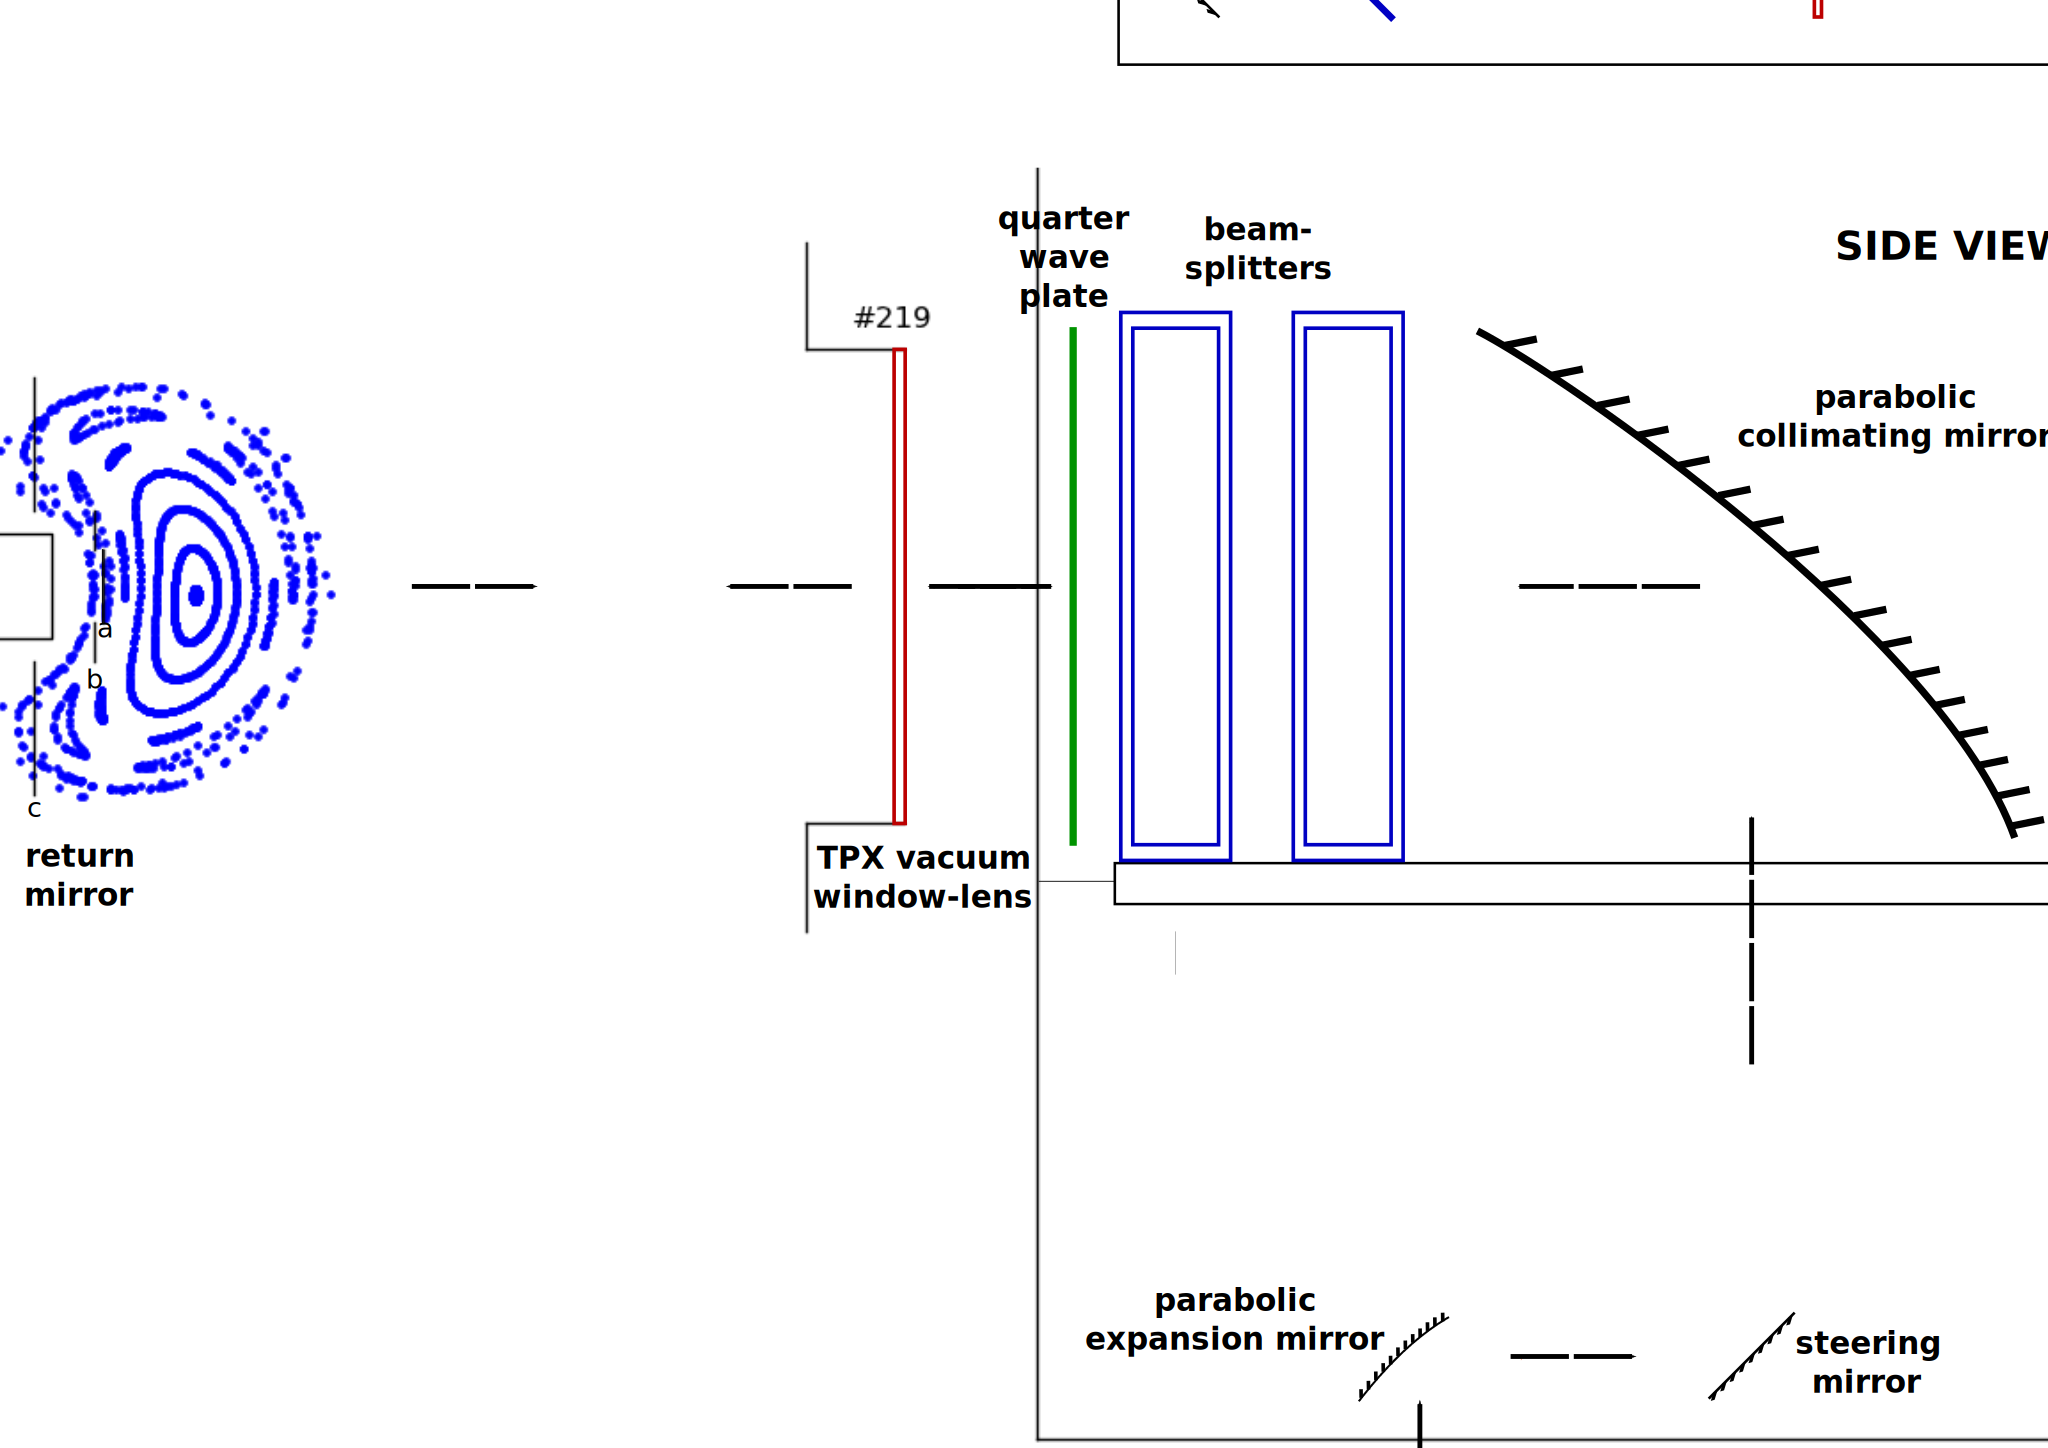
\includegraphics[width=\columnwidth]{figures/optical_component_layout_phaseii}
\caption{Overview of the optical layout.}
\label{fig:overview_schematic}
\end{figure}

\subsection{Gaussian beam modeling and FDTD simulations}
%FG & BDB
Beam dynamics may also be of value, possibly including FDTD simulations. Fresnel lens, quarter-wave plate, and imaging.
\thispagestyle{empty}
%Layout and components including mirrors, lens design, beamsplitter
%details and detector array.
%Beam dynamics may also be of value.
%Cover imaging arrangement, possibly including FDTD simulations.
\subsubsection{Beam modeling}


\subsubsection{FDTD simulations}


\label{sec:interferometer_design}

\section{Interferometer Components}
\thispagestyle{empty}
%Layout and components including source, mirrors, lens design, beamsplitter
%details, detectors, and detector arrangement.
\subsection{Fresnel lens}
The physical constraints of installing a full-view imaging interferometer on
the H-1 heliac requires imaging lenses with focal lengths $\approx 600
- 800$mm and diameters (or cross-section thereof) $\approx
600$mm.
For typical construction materials such as polymethylpentene
(PMP, also known as TPX) ($n_{\rm PMP} = 1.465$) and high density
polyethylene ($n_{\rm HDPE} = 1.53$), radii of curvature of $300 -
400$mm are needed, resulting in extremely large centreline thicknesses and
attentuation.
To satisfy these constraints---and after initially evaluating imaging properties\cite{MAHON2011}---a Fresnel lens design was chosen.
The lens has been precision machined from a single piece of PMP.
\begin{figure}[htbp]
\includegraphics[width=\columnwidth]{figures/fresnel_lens_detail}
\caption{Detail of the centre portion of the cylindrical Fresnel lens,
  seen from the side. The pyramidally-textured surface machined into
  the plane side of the lens reduces reflection.}% See \S \ref{sec:antiref_techniques}.}
\label{fig:antiref_photo}
\end{figure}

\subsection{Free-wire Beamsplitter}
High performance beamsplitters in the millimeter-wave range can be
constructed using a grating approach with closely-spaced, thin,
conductive wire, though this can prove challenging for large aperture optics.
For $\lambda \gg r$ (the radius of the wire), the co-efficient of reflection of the grating is given by
\cite{CASEY1952, RENK1962}
\begin{equation}
R = 1 - \left[ \frac{2d}{\lambda} \ln (\frac{d}{2 \pi r}) \right] ^2
\label{eq:beamsplitter_trans}
\end{equation}
and absoprtion by
\begin{equation}
A = \frac{d}{\pi r} \left[ {\frac{c}{\sigma \lambda}} \right]
^{\frac{1}{2}} R
\label{eq:beamsplitter_abs}
\end{equation}
where $d$ is the wire spacing, $\sigma$ is conductivity of the wire,
and $c$ is the speed of light.
For tungsten wire with $r = 5$\ts{}$\mu$m, a wire separation $d =
70$\ts{}$\mu$m, and $\sigma = 1.89 \times 10^7$\ts{}S/m

Meeting the challenge of a large aperture beamsplitter required
support frames suitable to meet the tension from many, closely-spaced
wound wires together with a metal-working lathe sufficiently large to
wind the beamsplitter.
Two support frames were bolted together, back-to-back, mounted and
turned slowly on a suitable lathe, winding $\approx 4000$\ts{}m of
tungsten wire over the pair.
Wires are glued to the frame, a securing clamping frame is attached
and the wires along the coupled frames' edges are cut, separating the
two beamsplitters.

For an incident wave polarized perpendicular to the wires the
beamsplitter is nearly completely transparent while waves polarized
parrallel are partially transmitted and partially reflected.\cite[p.280]{MARCUVITZ1951}
Thus, for a wave launched with polarization at 45\degrees{} to
horizontal wires, the reflected wave will be nearly completely
horizontally polarized and the transmitted wave a mix of both vertical
and horizontal polarizations.
The second beamsplitter thus reflects the horizontally-polarized
`leaked' component of the wave transmitted from the first beamsplitter
and a beam dump is installed on the vertical support table to suppress
reflection of this wave back into the optical path.

\subsection{Quarter-wave Plate}
The optical layout and power efficiency of the interferometer design
is dependent on a suitably performing quarter-wave plate. Various designs
of form birefringent components exist\cite{VANVLIET81} allowing
flexibility in the design of a suitable wave plate. 

\subsection{Anti-reflection Techniques}
\label{sec:antiref_techniques}
Reducing the contribution of minor reflection cavities within the
optical layout to the final interferogram is a priority in improving
the reliability of the measurement of the phase shift in the probe arm
and, hence, the electron density measurements.
One technique to reduce these contributions is to tilt the optical
components from normal incidence such that the initial pass of the
beam through them is relatively undisturbed but subsequent
reflections, say from the next optical component, are reflected out of
the beam path.
The vacuum window-lens, shown in Figure \ref{fig:overview_schematic},
has such a tilt along the longtitudinal axis permanently integrated as
part of the lens design.
Other lenses, such as the imaging and detector focussing lenses, are
able to be rotated longtitudinally as part of their mounting system.
To further reduce unwanted reflections within the system a pyramidally
textured surface\cite{DEINEGA2010} is machined into the plane side
of each lens, as shown in Figure\ref{fig:antiref_photo}.
The pyramid peaks are spaced 2\ts{}mm apart with a peak-to-base depth
of 2.6\ts{}mm.

\label{sec:interferometer_components}

\section{Modulation strategies}
\thispagestyle{empty}
%SRH
%The sinusoidal drive of the source and subsequent demodulation including performance.
\subsection{Linear/sawtooth modulation}
Initially, a sawtooth phase modulation technique was used.
By carefully selecting the modulation depth so that the difference between the wavelength at the lowest frequency and highest frequency correspond to exactly an integer multiple of the path length difference between the probe and reference arm, this technique is essentially the same as providing a linear phase ramp.
This has the benefit of being relatively simple to demodulate by calculating the argument of the Hilbert transform of the modulated signal, following appropriate filtering of the signal.
The frequency response of this modulation scheme is limited by the achievable $\delta \omega / \delta t$ of the source, preventing the use of sawteeth with frequencies above 20kHz and consquently reducing the maximum bandwidth of the system to $\sim10$kHz. 

While this is acceptable for looking at the slow time evolution of the plasma density, it is not very useful for looking at fluctuations such as Alfven waves, many of which have frequencies up to 40kHz on H-1NF.
To increase the bandwidth of the system to see these fluctuations, a sinusoidal modulation scheme was used.
\subsection{Sinusoidal modulation}
\begin{equation}
\label{eqn:probe_output1}
I(t) = \frac{I_0}{2} (1 + \zeta \cos(\phi_0 + \phi_1 \sin(2 \pi f_M t))
\end{equation}
Which can be represented as follows where $\Gamma=\Gamma_c+i \Gamma_q=\zeta\cos(\phi_0)+i\zeta\sin(\phi_0)$:
\begin{equation}
\label{eqn:probe_output2}
I(t) = \frac{I_0}{2} \{1 + \Gamma_c \cos[\phi_1 \sin(2 \pi f_M t + \epsilon)] - \Gamma_q \sin[\phi_1 \sin(2 \pi f_M t + \epsilon)]\}
\end{equation}
By using the following identities:
\begin{align}
\label{eqn:probe_output3}
\sin [z \sin (\theta)] &= 2 \sum_{k=0}^{\infty} J_{2k +1} (z) \sin [(2k+1) \theta]~, \\
\cos [z \sin (\theta)] &= J_0 (z) + 2 \sum_{k=0}^{\infty} J_{2k} (z) \cos (2k \theta)~,
\end{align}
where $J_n$ is the Bessel function of the nth order, this equation to be rewritten as:
\begin{equation}
\label{eqn:probe_output4}
\begin{split}
I(t) = \frac{I_0}{2} \{1 + \Gamma_c \sum_{k=-\infty}^{\infty} J_{2k} (\phi_1) \cos [2k (2 \pi f_M t + \epsilon)] - \\
\Gamma_q \sum_{k=-\infty}^{\infty} J_{2k +1} (\phi_1) \sin [(2k+1)(2 \pi f_M t + \epsilon)]\}~.
\end{split}
\end{equation}
Taking the Fourier transform:
\begin{align}
\begin{split}
\label{eqn:fourier_representation}
\mathcal{I} (f) = &\sum_{k=-\infty}^{\infty} J_{2k} (\phi_1) \frac{1}{2} [\exp (2k i \epsilon) (\mathcal{C}(f - 2 k f_m))] + \\
&\frac{i}{2} \sum_{k=-\infty}^{\infty} J_{2k+1} (\phi_1) \mathcal{Q}(f - (2k+1) f_m) \exp [i(2k +1 ) \epsilon]~,
\end{split}
\end{align}
results in a series of harmonics that are multiples of the source frequency modulation frequency. We want to extract $\Gamma_c (t)$, $\Gamma_q (t)$, but to do that we need to obtain $\phi_1$ and $\epsilon$.


%The sinusoidal drive of the source and subsequent demodulation including performance.

\label{sec:modulation_strategies}

\section{System Characterization}
\thispagestyle{empty}
% FG & SRH
%Object space imaging and phase characterisation results.

Several bench top tests were performed to quantify the performance of the interferometer multi-path issues, . These tests fall into  , and tests for consistency between the sawtooth and sinusoidal source modulation.

\subsection{Interference tests}
To test the performance of the interferometer, the interferograms were recorded with both the probe and reference arm open, only the probe arm open and only the reference arm open.
For the cases where a single arm is open, only a DC offset should be observed in the detector signals; however, the presence of unwanted reflections (multi-path) within the system gives rise to interference, which leads to errors when both arms are open.
The extent of these problems is examined by checking the RMS of the AC component of the detector outputs, with various arms open (figure~\ref{fig:RMS_interference}).

\begin{figure}[!h]
\begin{center}
\includegraphics[]{figures/interference.pdf}
\end{center}
\caption{(a) RMS of the interferograms with various interferometer arms open for all of the interferometer channels. The variation in the amplitude with channel is due to different detector sensitivities and the Gaussian shape of the beam. (b) Ratio of the RMS from the single arms to both arms, highlighting the extent to which multi-path is a problem for each channel.}
\label{fig:RMS_interference}
\end{figure}

\subsection{Imaging Tests}
Stainless steel mirrors were manufactured with shallow sine waves machined into their surface to act as phase objects.
The wavelength and peak to peak depth of the sine waves for the different mirrors were: (wavelength$~=100\mathrm{mm}$,depth$~=1\mathrm{mm}$), ($100\mathrm{mm}$,$0.5\mathrm{mm}$), and ($60\mathrm{mm}$,$0.5\mathrm{mm}$).
The machining tollerance of these mirrors was measured to be within $10\mu\mathrm{m}$.
By placing these mirrors on a motorised vertical stage in the imaging plane, the imaging behaviour of the interferometer can be tested.
Figure~\ref{fig:moving_mirror_contour} shows one such tests with the ($100\mathrm{mm}$,$1\mathrm{mm}$) mirror, where at $t\approx5\mathrm{s}$ the mirror starts moving upwards, at $t\approx24\mathrm{s}$ the motorised stage stops before moving back downwards at $t\approx29\mathrm{s}$ (note the image is inverted at the detector array).

\begin{figure}[!h]
\begin{center}
\includegraphics[]{figures/shot-85368-wavelength-100-depth-1-00pi-contour.pdf}
\end{center}
\caption{}
\label{fig:moving_mirror_contour}
\end{figure}

As the mirror moves vertically, the demodulated output from the $i^{\mathrm{th}}$ detector can be modelled as:
\begin{equation}
\label{eqn:wobbly_mirror_fit}
p_i(t) = A_i \sin(k x_i - \omega t + \phi)~~,
\end{equation}
where $\phi$ is an initial phase offset due to the starting position of the mirror, $A_i$ is the depth of modulation observed by the detector which should be the same across all channels, $k$ is the wavenumber of the sinusoidal modulation machined into the mirrors including any magnification due to the imaging system, $\omega$ is a function of the wavelength of the mirror and how quickly the motorised stage is moving, and the detectors location is given by $x_i$.

The demodulated signal from each channel should reproduce the sine that is created due to the path length change as the mirror moves upwards.
Additionally, each channel will see an initial phase in the sine wave, with the relationship between these initial phases across the channels representing the spatial structure of the wobbly mirror. 
Figure~\ref{fig:moving_mirror_amp_phase} shows the amplitudes and initial phases for the three different phase objects. 
The variation in the observed amplitude between the different channels is due to the multi path issues that have been described earlier.

\begin{figure}[!h]
\begin{center}
\includegraphics[]{figures/85368_85372_85391_k-amp.pdf}
\end{center}
\caption{(a) Plot of the initial phase for vertically subsequent detectors ($kx_i$ in equation~\protect\ref{eqn:wobbly_mirror_fit}). As the $k$ of a particular wobbly mirror is fixed, and $x_i$ are evenly spaced, the values are expected to form a straight line. The solid lines show the expected trend based on the dimensions of the mirrors and the speed of the stage. (b) Plots of $A_i$ to check for consistency in the observed depth across the detector channels.}
\label{fig:moving_mirror_amp_phase}
\end{figure}

To test the depth of field of the imaging system, the location of the wobbly mirror is moved through the focal plane, with measurements of the observed depth of the sinusoidal modulation recorded across all of the channels at specific discrete locations.
Figure~\ref{fig:depth_of_field} demonstrates that is a strong maximum in the data as the mirror approaches the focal plane demonstrating the imaging....
\begin{figure}[!h]
\begin{center}
\includegraphics[]{figures/depth_of_field.pdf}
\end{center}
\caption{}
\label{fig:depth_of_field}
\end{figure}


\label{sec:system_characterization}

\section{Plasma Results}
\thispagestyle{empty}
Include some juicy `typical' data showing off the bandwidth and spatial coverage of the system.

\label{sec:plasma_results}

\acknowledgments
The authors would like to thank the H-1NF team for continued support
of experimental operations.
This work was supported by the Education Investment Fund under the
Super Science Initiative of the Australian Government.

\bibliographystyle{plain}
\bibliography{references}


\end{document}
